\chapter{Grundlagen}\label{kap:grundlagen}

%####################  CHAPTER 1: Grundlagen  #################

Das vorliegende Kaptitel beschreibt zunächst die Grundlagen des Machine 
Learnings, mit Neuronalen Netzen allgemein und anschließend im 
Einsatz des maschinellen Sehens.

Desweiteren wird die für die Inferenz, verwendete Hardware, 
der Neural Compute Stick 2 vorgestellt.


%------------------- SECTION: Machine Learning ------------------

\section{Machine Learning}\label{sec:ml}

Beim Machine Lerining, welches ein Teilgebiet der Computerwissenschafen
ist, geht es um die Erstellung von Algorithmen, die Zusammenhänge in großen
Datenmengen erkennen, ohne explizit darauf programmiert worden zu sein.

Eine Form davon ist das \textit{Supervised Learning}, bei dem das Programm 
neben den Input Daten auch die Zugehörigen Ausgaben erhält und daraus 
dann die Regeln für Zusammenhänge ableiten soll.
Dadurch unterscheidet sich das Vorgehen wesentlich zur klassischen Programmierung,
bei bei der die Regeln vorab definiert werden müssen.


% \vspace{0.5cm}
% \begin{figure}[htb]
%     \centering
%     \def\svgwidth{0.8\columnwidth}
%     \footnotesize
%     
\tikzset{
    decision/.style={
        diamond,
        draw,
        text width=4em,
        text badly centered,
        inner sep=-1pt,
        node distance=8em
    },
    block/.style={
        rectangle,
        draw,
        text width=6em,
        %minimum widhth=6em,
        minimum height=5em,
        text centered,
        node distance=20em
    },
    arrow/.style={
        draw,
        >=latex,
        ->
    },
    textfeld/.style={
        %draw,
        text centered,
        node distance=1.5em
    }
}


\begin{tikzpicture}

    
    \node (system) [block] {Klassisches\\Programm};
    \node (system2) [block, right of=system] {Machine Learning\\Programm};

    \node [textfeld, left=of system.162] (inputs) {Daten};
    \node [textfeld, left=of system.198] (regeln) {Regeln};
    \node [textfeld, right=of system] (output) {Ausgaben};

    \node [textfeld, left=of system2.162] (inputs2) {Daten};
    \node [textfeld, left=of system2.198] (output2) {Ausgaben};
    \node [textfeld, right=of system2] (regeln2) {Regeln};
    
    \draw[arrow] (inputs) -- (system.162);
    \draw[arrow] (regeln) -- (system.198);
    \draw[arrow] (system) -- (output);
    
    \draw[arrow] (inputs2) -- (system2.162);
    \draw[arrow] (output2) -- (system2.198);
    \draw[arrow] (system2) -- (regeln2);
    

\end{tikzpicture}

% \end{figure}
% \vspace{0.5cm}



Das ableiten der Regeln erfolgt beim Machine Learning in einem 
iterativen Prozess, welcher als Training bezeichnet wird.
Dabei werden die Zusammenhänge zwischen In- und Output Daten 
als mathematische Funktion betrachtet, welche numerisch 
angenähert wird.

Bei einem linearen Zusammenhang, handelt es sich
um eine Regression und bei einem kategorischen um 
eine Klassifizierung.


Weitere Formen neben dem \textit{Supervised Learning} sind das 
\textit{Unsupervised Learning}, bei der das Programm keine Labels 
erhällt, sondern diese durch Clustering Verfahren selber finden 
soll, oder das \textit{Reinfocement Learning}, bei dem das Programm 
mit der Umwelt interagieren soll.
\\
Diese techniken wurden in der Bachelor Arbeit nicht verwendet 
und werden daher nicht näher erläutert.

%------------------- SECTION: Neuronale Netze -------------------

\subsection{Künstliche Neuronale Netze} \label{subsec:nn}

Für komplexe Input Daten, wie beispielsweise Bilder, bei denen 
die einzelnen Pixelwerte als Inputs und der Inhalt des Bildes als 
Output dienen, werden in der Regel künstliche Neuronale Netze verwendet.
Diese sind eine Form des Machine Learings und bestehen aus einer 
vielzahl an miteinander verbundener Neuronen. Durch unterschiedlich 
starke Gewichtungen der einzelnen Verbindungen, auch Gewichte genannt, 
können für unterschiedliche Input Daten die entsprechenden Outputs 
gefunden werden.

\begin{figure}[htb]
    \centering
    \label{fig:nn}
    \def\svgwidth{0.5\columnwidth}
    \footnotesize
    \begin{neuralnetwork}[height=1]
    \newcommand{\nodetextclear}[2]{}
    \newcommand{\nodetexth}[2]{$h_#2$}
    \newcommand{\nodetextx}[2]{$x_#2$}
    \newcommand{\nodetexty}[2]{$y_#2$}
    \inputlayer[count=3, bias=false, title=Input\\layer, text=\nodetextx]
    \hiddenlayer[count=4, bias=false, title=Hidden\\layer, text=\nodetexth] \linklayers
    \outputlayer[count=2, title=Output\\layer, text=\nodetexty] \linklayers
\end{neuralnetwork}
\end{figure}


Die richtige Einstellung der Gewichte, welche zunächst zufällig initialisiert werden, 
erfolgt dabei im Trainingsprozess, welcher in \ref{fig:train} schematisch
 dargestellt ist aus folgenden drei Schritten besteht.

\begin{itemize}
    \item \textit{Forward Pass} anhand aktueller Gewichte vorhersage aus den Inputs treffen
    \item \textit{Fehlerbestimmung} Abweichung zum tatsächlichen werten berechnen
    \item \textit{Backpropagation} minimierung der Fehlerfunktion durch Anpassung der Gewichte
\end{itemize}

\begin{figure}[htb]
    \centering
    \label{fig:train}
    \def\svgwidth{0.5\columnwidth}
    
\tikzstyle{process} = [rectangle, fill=blue!20, minimum width=2.5cm, minimum height=1cm, text centered, draw=black]
\tikzstyle{arrow} = [thick,->,>=stealth]

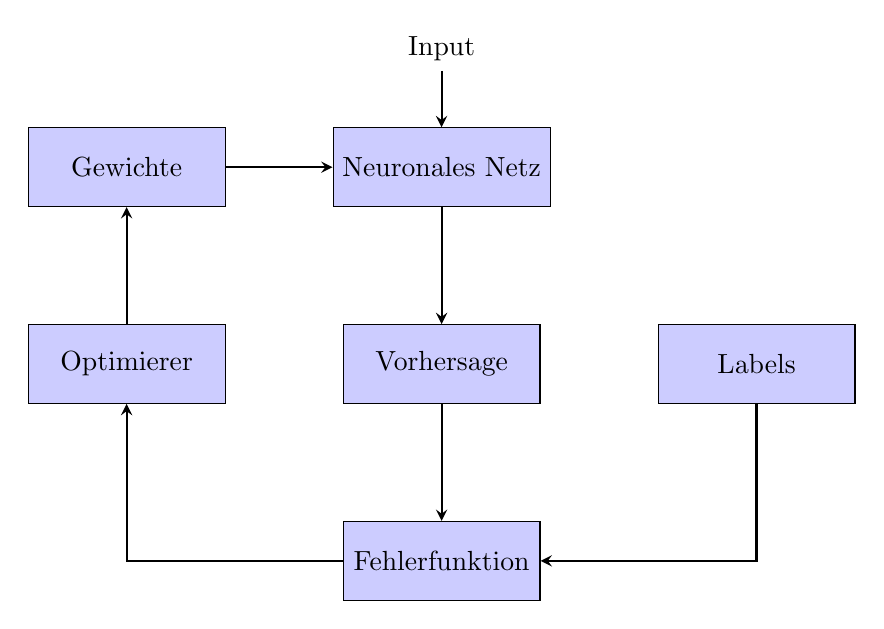
\begin{tikzpicture}[node distance=1.6cm]

  \begin{scope}[node distance=2.5cm]
    \node (nn)      [process]                   {Neuronales Netz};
    \node (pred)      [process, below of=nn]      {Vorhersage};
    \node (loss)      [process, below of=pred]      {Fehlerfunktion};
    
  \end{scope}
  
  \begin{scope}[node distance=4cm]
    \node (opt) [process, left of=pred]      {Optimierer};
    \node (weights)  [process, left of=nn] {Gewichte};
    \node (labels)   [process, right of=pred]  {Labels};
  \end{scope}

  \node (input) at (0,1.5) {Input};

  \draw[arrow] (input) -- (nn);

  \draw[arrow] (nn) -- (pred);
  \draw[arrow] (pred) -- (loss);

  \draw[arrow] (labels) |- (loss);
  \draw[arrow] (loss) -| (opt);

  \draw[arrow] (opt) -- (weights);
  \draw[arrow] (weights) -- (nn);
  
    
\end{tikzpicture}

    \caption{Trainingsablauf NN}
\end{figure}

Durch merhfaches durchlaufen der Schritte wird die Fehlerfunktion soweit minimiert, 
sodass das Modell auch für neue Input Daten die richtigen Aussagen treffen kann.


\subsubsection{Forward Pass}
Im \textit{Forward Pass} werden die Inputs durch alle Schichten hindurch 
gereicht, um in der letzten Schicht den gewünschten Output zu liefern.
Dabei erhält jedes Neuron die mit $w_{i}$ gewichteten Ausgabewerte aller
Neuronen der vorherigen Schicht und summiert diese zusammen mit einem konstanten 
Bias Wert $b$ auf. 
Mithilfe einer Aktivierungsfunktion wird der Wert auf eienen bestimmenten Bereich 
skalliert \ref{fig:neuron}


\begin{figure}[h]
    \centering
    \label{fig:neuron}
    \begin{tikzpicture}[
    % define styles    
    init/.style={ 
         draw, 
         circle, 
         inner sep=2pt,
         font=\Huge,
         join = by -latex
    },
    squa_draw/.style={ 
        draw,
        font=\Large,
        join = by -latex
    },
    squa/.style={ 
        font=\Large,
        join = by -latex
    }
]
% Top chain x1 to w1
\begin{scope}[start chain=1]
    \node[on chain=1] at (0,1.5cm)  (x1) {$x_1$};
    \node[on chain=1,join=by o-latex] (w1) {$w_1$};
\end{scope}
% Middle chain x2 to output
\begin{scope}[start chain=2]
    \node[on chain=2] (x2) {$x_2$};
    \node[on chain=2,join=by o-latex] {$w_2$};
    \node[on chain=2,init] (sigma) {$\displaystyle\Sigma$};
    \node[on chain=2,squa_draw,label=below:{\parbox{2cm}{\centering Aktivierungs\\ Funktion}}]   {$\delta(z)$};
    \node[on chain=2,squa,label=below:Output,join=by -latex] {$y_{out}$};
\end{scope}
% Bottom chain x3 to w3
\begin{scope}[start chain=3]
    \node[on chain=3,label=below:Inputs] at (0,-1.5cm) 
    (x3) {$x_3$};
    \node[on chain=3,label=below:Gewichte,join=by o-latex]
    (w3) {$w_3$};
\end{scope}
% Bias
\node[label=above:\parbox{2cm}{\centering Bias \\ $b$}] at (sigma|-w1) (b) {};
% Arrows joining w1, w3 and b to sigma
\draw[-latex] (w1) -- (sigma);
\draw[-latex] (w3) -- (sigma);
\draw[o-latex] (b) -- (sigma);

\end{tikzpicture}

% von https://medium.com/momenton/typesetting-neural-network-diagrams-with-tex-4920b6b9fc19
    \caption{Einzelnes Perzeptron}
\end{figure}



Um den Forward Pass für eine gesmmte Schicht, besthend aus 
einer Vielzahl an Neuronen, zu berechnen, werden die Schichten 
als Vektren und die Gewichte als Mtrizen dargestellt.
\\
Die Matrixmultiplikation aus dem Vektor der vorherigen 
Schicht $x$ der Gecwichtsmatrix $W$ ergibt die Werte des Vektors 
der aktuellen Schicht,


\begin{equation}
    \label{eq:forward}
    z = W^{T}x+b
\end{equation}

welcher anschließend elementweise einer nichtlinearen Aktivierungsfunktion
$g(z)$ übergeben wird.\\
Für mittlere Schichten wird dabei oft die in \ref{eq:relu} dargestellte
\textit{ReLU} verwendet eine Funktion die negative Werte zu 0 setzt.

\begin{equation}
    \label{eq:relu}
    g(z) = max\{0,z\}
\end{equation}

Da die Ausgabe meist einen Wahrscheinlichkeites Wert zwischen 0 und 1 
Um für die Outputs einen Wahrscheinlichkeits Wert zwischen 0 und 1 
zu erhalten, wird an der Ausgabeschicht für eine binäre Klassifikation 
die Sigmoid Funktion (\ref{eq:sidmoid}) verwendet,
welche S-Förmig zwischne 0 und 1 verläuft.

\begin{equation}
    \label{eq:sidmoid}
    g(z) = \frac{1}{1 + e^{-x}}
\end{equation}


Für eine Kategorische Ausgabe mit mehr als zwei Werten wird 
die Softmax (\ref{eq:softmax}) Funktion verwendet, welche eine Wahrscheinlichkeits 
Verteilung über alle Ausgebe Neuronen generiert.

\begin{equation}
    \label{eq:softmax}
    g(z) = \frac{e^{z}}{\sum e^{x}}
\end{equation}


\subsubsection{Fehlerbestimmung}
Die Abweichung der Schätzung, welche an den Neuronen der letzen Schicht 
vorliegen, zu den tatsächlichen Werten, den Labels, wird mithilfe einer geeigneten
Fehlerfunktion bestimmt. Für die lineare Regression wird dabei z.B. 
der absolute oder quadratischen Abstand verwendet, für ein 
Klassifizierungs Modell ist jedoch eine logarithmische Fehlerberechnung 
mit der Cross Entropy Funktion, in \ref{eq:crossentropy} dargestellt effektiver.


 \begin{equation}
    \label{eq:crossentropy}
    L = \hat{y}log(y) + (1 - \hat{y})log(1 - y)
\end{equation}

Durch den Logarithmus wird der Loss um so größer, je weiter die Schätzung $y$ vom 
tatsächlichen Wert $\hat{y}$ abweicht.
%hier plot


\subsubsection{Backpropagation}

Durch Berechnung des Gradienten der Fehlerfunktion kann ermittelt 
werden in welche Richtung die Gewichte angepasst werden müssen, sodass diese sich 
im nächsten Durchgang minimiert.

Dafür wird die die Fehlerfunktion $L$ für jede Schicht partiell nach den 
Gewichten $w$ abgeleitet, was wie in gl. \ref{eq:backprop} dargestellt mithilfe der 
Kettenregel über die Aktivierungsfunktion $z$ geschieht.


\begin{equation}
    \label{eq:backprop}
    \frac{\partial L}{\partial w} = \frac{\partial L}{\partial z}\frac{\partial z}{\partial w}
\end{equation}
Mit dem ermittelten Gradienten werden dann die Gewichte nach Gleichung \ref{eq:update_wieghts} angepasst.
\begin{equation}
    \label{eq:update_wieghts}
    w  \leftarrow w - \eta \frac{\partial L}{\partial w}
\end{equation}

wobei die \textit{Lernrate} $\eta$ die Schrittweite ist, mit der die
Anpassungen vorgenommen werden.





%------------------- SUBSECTION: Validierung -------------------
\subsection{Validierung und Overfitting}\label{subsec:validation}

Um überprüfen zu können, ob und wie gut ein Modell die Zusammenhänge
in den Trainingsdaten generalisiert hat, dh auch für neue Daten
anwendbar ist,
wird der Datensatz in einen Trainings- und einen Testdatensatz aufgeteilt.

Während des Trainings wird für beide Sätze der Fehler berechnet, 
die korrektur der Gewichte mittels Backpropagation erfolgt
jedoch nur anhand der Trainingsdaten.

Entsteht eine Abweichung der beiden Fehlerfunktion wie in 
[plot overfitting] dargestellt, findet eine Überanpassung 
an die trainingsdate \textit{Overfitting} statt.

Gründe dafür sind zu wenig Trainingsdaten oder ein zu komplexes Model, 
welches sich ähnlich einer polynomialen Funktion mit hohem Grad 
an jeden datenpunkt anpassen kann, damit kein generalisierbare 
Aussage für neue Daten mehr getroffen werden kann.


\begin{figure}[htb]
    \centering
    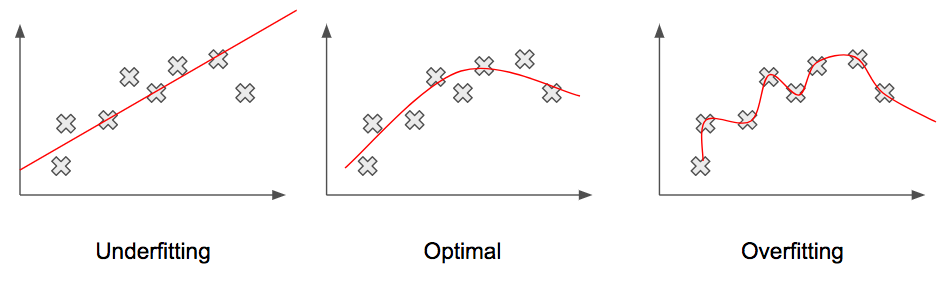
\includegraphics[width=0.8\textwidth]{over_under_fit.png}
    \caption{Quelle: \cite{deshpGuideImprovingDeep2017a}}
    \label{fig:over_under_fit}
\end{figure}

% Overfitting -> hohe varianz: varianz = train_err - test_error
% Underfitting -> hoher Bias: Bias = 

Um Overfitting, auch wenn nicht mehr Trainingsdaten 
zur Verfügung stehen zu vermeiden, gibt es verschiedene
Techniken:\\\\
\textit{Augmentierung}\\
Bei Augmentierung werden aus den vorhandenen Daten künstlich mehr 
Daten generiert, in dem an den Bildern geometrische transformationen 
oder manipulationen der pixelwerte vorgenommen werden.
\\\\
\textit{Regularisierung der Parameter (L1/L2)}\\
Bei Regularisierung wird an die Lossfuction als weiterer Term
 eine aufsummierung der Gewichte gehängt, wodurch diese bei der Minimierung 
  klein gehalten werden, wodurch weniger potential zur überanpassung da ist.
  \begin{equation}
    \label{eq:regularization}
    J(w) = E + \lambda \sum_{i} w_{i}^{2}
\end{equation}
\textit{Dropout}\\
Beim Dropout werden zufällig gewichte zu 0 gesetzt.
\\\\
\textit{Early Stopping}\\
stoppen des trainings, wenn sich overfitting einstellt.



\section{Computer Vision}

Deep Learning + Techniken der Bildverarbeitung

%---------------- SUBSECTION: Convolutional ----------------
\subsection{Convolutional Neural Networks}\label{subsec:cnn}

Convolutional Neural Networks sind eine Erweiterung 
der in \ref{sec:nn} beschriebenen Neuronalen Netze 
und besonders geeignet für die Bilderkennung.

Befor die Klassifizierung mittels Fully Connected Network 
stattfindet, sollen für die Klasse spezifische Merkmale 
aus dem Input Bild heraus extrahiert werden.

Dafür werden über das Bild zeilenweise Filtermatrizen mit kleinerer Dimension
(3x3, 5x5) geschoben und eine math Faltung angewendet.
Die Ergebnisse der Faltungen ergeben eine sog Feature Map, in welcher 
Muster die sowol in Filter Mtrix als auch in input Bild auftreten, verstärkt 
dargestellt werden.

Die Werte der Filter Matrizen entsprechen den zu lernenden Gewichten 
und werden mithilfe der Backpropagation angepasst.

\begin{figure}[htb]
    \centering
    \label{fig:conv}
    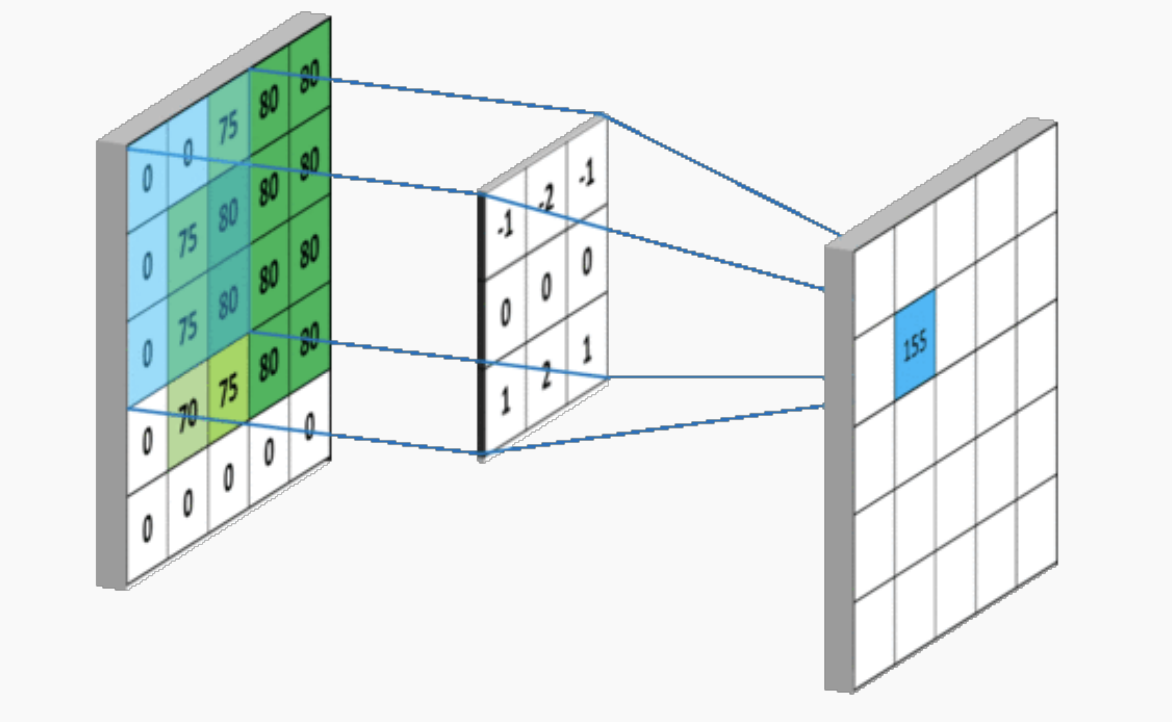
\includegraphics[width=0.4\columnwidth]{convolution.png}
    \caption{Faltung, \cite{researcherSimpleIntroductionConvolutional2019}}
\end{figure}



Durch die hintereinanderschaltung mehrerer Convolutional Layern 
lassen sich so immer komplexere Merkmale des Input Bildes in den 
Feature Maps heraus extrahieren.

Durch Subsampling Methoden wie Max Pool Layer zwischen den Convolutional
Layern verkleinert sich die Dimension der Ferture Maps in jeder Schicht.


\begin{figure}[htb]
    \centering
    \label{fig:lenet}
    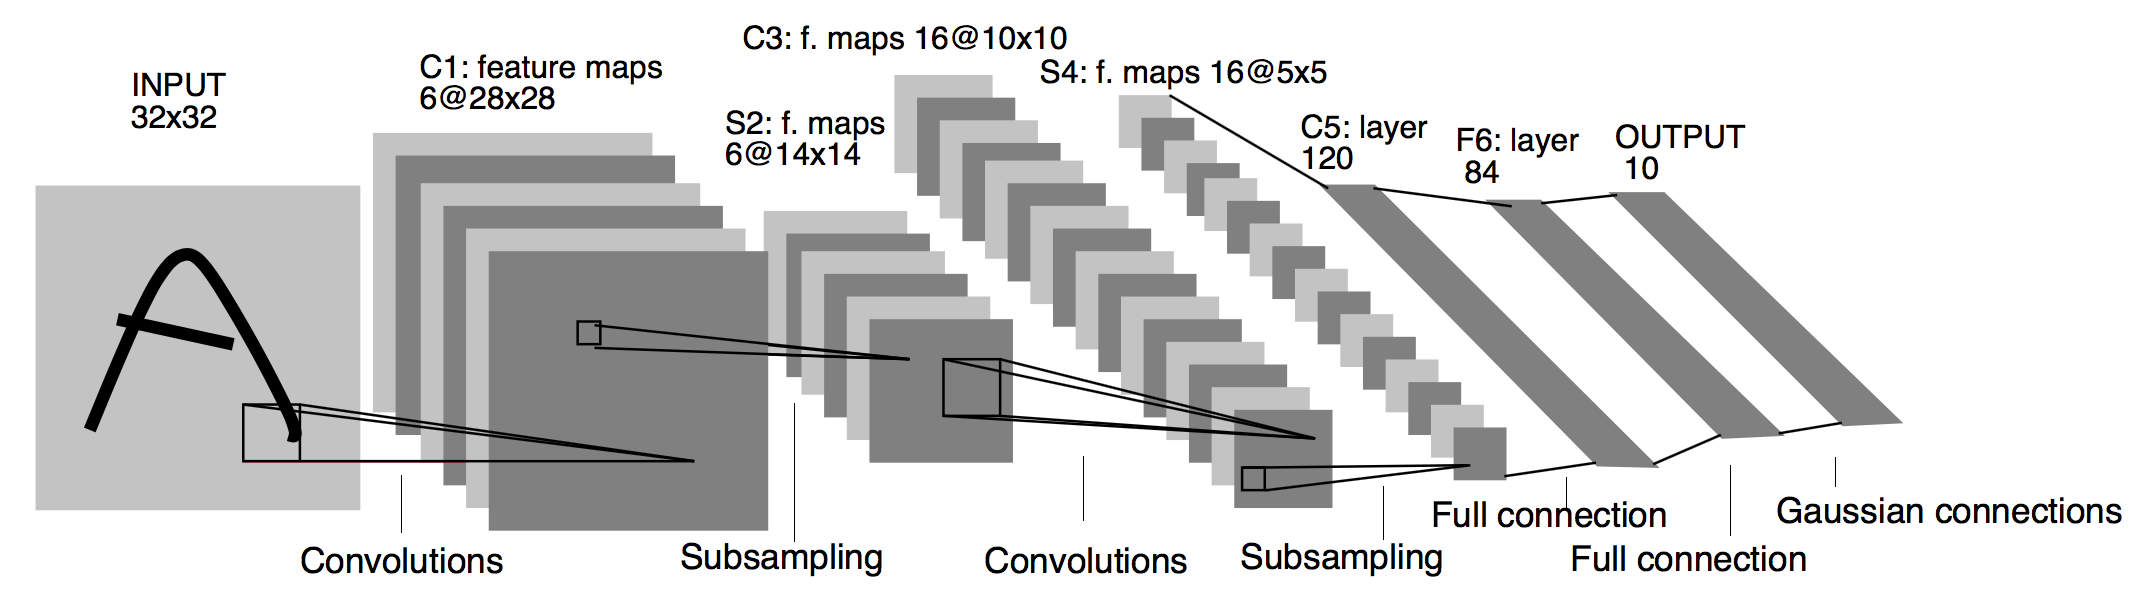
\includegraphics[width=0.8\columnwidth]{lenet.png}
    \caption{Faltung, \cite{lecunGradientBasedLearningApplied1998}}
\end{figure}


Vorteile der CNNs sind der geringere Rechenaufwand durch die gemeinsame 
Nutzung der Paramer der Filter Matrizen und die durch die 
Faltung zustande kommende räumliche invarianz für das zu erkennende 
Objekt auf dem Bild.
\\
Um die Features, welche insbesondere in den vordersten ConvLayern für 
alle klassen sehr ähnlich sind, nicht bei jedem Modell
neu lernen zu müssen, wird häufig \textit{Transfer Learing} angewendet, 
d.h. es werden die auf ein allg Datenset wie z.B. ImageNet vortrainierten
Gewichte verwendet und müssen so nur noch etwas für den eigenen Datensatz 
fine getuned werden.


\subsubsection{Architkturen}\label{subsubsec:architecture}

Nach der in Abbildung \ref{fig:lenet} dargestellten, erfolgreichen
ersten veröffentlichung eines CNN von YannLecunn 1998 \cite{lecunGradientBasedLearningApplied1998}
wurden wurden viele weitere Architekturen entwickelt. 

Diese werden anhand der ImageNet Chanllange ILSVRC \cite{ILSVRC15} bewerted

Die bekanntesten gewinner Modelle sind wie in \cite{StanfordCS231nConvolutional}
aufgeführt:


\begin{itemize}
    \item Alexnet (2012), mehrere conv layer hintereinander
    \item GoogleLeNet (2014), Inception Module
    \item VGGNet 2014
    \item ResNet (2015), 
\end{itemize}

%---------------- SUBSECTION: Obj Detection ----------------
\subsection{Objekt erkennung}\label{subsec:objdet_det}

Neben der Information, was sich auf einem Bild befindet möchte
man bei der Object Detection auch herausfinden wo sich das 
Objekt befindet.
Dafür wird ein in \ref{subsec:cnn} beschriebenes CNN als Basis 
zusammen mit weiteren Mechanaismen, auf die in \ref{sec:related_work}
genauer eingegangen wird, verwendet.
\begin{figure}[htb]
    \centering
    \label{fig:class_vs_det}
    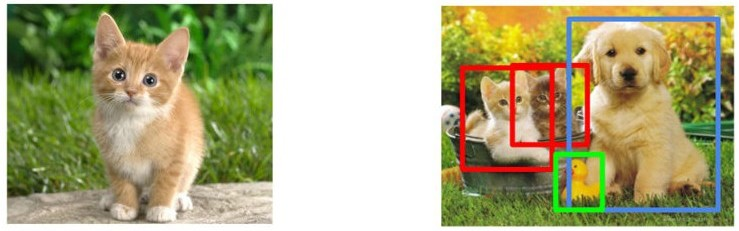
\includegraphics[width=0.8\textwidth]{classification_detection_small.jpeg}
    \caption{Unterschied: Classification - Detection}
\end{figure}


%------------------- SUBSECTION: ML Frameworks ---------------
\subsection{Deep Learing Lerining Frameworks}
\begin{itemize}
    \item Frameworks allgemein
    \item TensorFlow
\end{itemize}


%------------------- SECTION: Hardware ----------------------
\section{Neural Compute Stick 2}\label{ncs2}
%noch eine section zu Hardware allg (cpu, gpu, tpu), Neural Compute Stick und AI on the egde

Da das Training und die Inferenz von Deep Learning Algorithmen
 sehr rechenintensiv ist, werden entsprechen leistungsfähige 
Prozessoren benötigt. Dabei ist die Ausführung auf einer GPU 
(Graphical Processor Unit) meist effizienter als auf einer 
CPU (Central Processor Unit).

Anwendungen auf eingebetteten Systemen
wie z.B. einplatinen Computern wie dem in der Arbeite verwendeten
Raspberry Pi kommen dabei schnell an ihre Grenzen.
Möchte man dennoch die Daten auf dem Gerät verrechnen und 
nicht an eine Cloud senden, bieten verschiedene KI Beschleuniger 
die möglichketi die Inferenz des Deep Learning Modells 
auf externer Hardware auszuführen. Einer davon ist der in der 
Arbeit verwendete Neural Compute Stick 2 von Intel.
\\
Dieser basiert auf der Movidius Myriad X Vision Processing Unit (VPU)
\cite{haussermannFunktionUndEffizienz}

\begin{figure}[htb]
    \centering
    \label{fig:ncs2}
    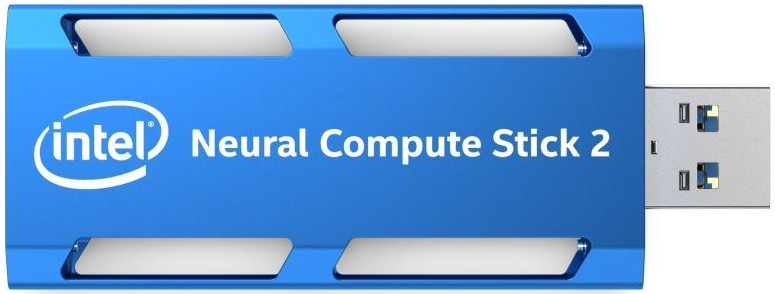
\includegraphics[width=0.4\columnwidth]{ncs2_top.jpg}
    \caption{NCS2}
\end{figure}


\subsection{OpenVino Toolkit}



% doku:
% https://docs.openvinotoolkit.org/latest/_docs_IE_DG_Introduction.html
% tutorial (mit guten diagrammen)
% Car
% https://github.com/intel-iot-devkit/inference-tutorials-generic/tree/openvino_toolkit_2019_r1_0/car_detection_tutorial#tutorial-step-3-add-the-second-model-vehicle-attributes-detection
% Face
% https://github.com/intel-iot-devkit/inference-tutorials-generic/blob/openvino_toolkit_2019_r1_0/face_detection_tutorial/Readme.md



Um die Inferenz eines trainierten Deep Learing Modells auf dem
Neural Compute Stick ausführen zu können, wird das Toolkit 
OpenVino verwendet.

Dieses ist eine Plattform zur Otimierung und Inferenz von 
CNN Basierten Modellen auf unterschiedlicher Intel Hardware.

Dabei wird ein eigenes Dateiformat verwendet, die \textit{Intermediate 
Representation} (IR), welche die Struktur/Architektur des Modells 
in einer .xml Datei und die trainierten Parameter/Gewichte in 
einer Binary (.bin) datei abbildet.

Mit dem \textit{Model Optimizer} können Modelle der Frameworks 
TensorFlow, Caffe, ONNX, Kaldi, oder MXNET in das IR Format 
konvertiert werden.

Um diese dann auf die entsprechende Hardware zu laden und anwendbar 
zu machen, wird die auch in OpenVino enthaltene \textit{InferenceEngeine}
verwendet.

Diese bietet eine Api mit der aus der Anwendung heraus in den 
Programmiersprachen C++ oder Python auf die Funktionen der 
InferenceEngeine zugegriffen werden können.

\begin{figure}[htb]
    \centering
    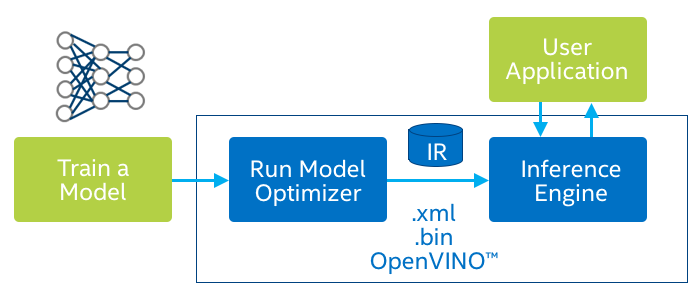
\includegraphics[width=10cm]{./Bilder/open_vino_workflow_steps.png}
    \caption{Workflow: OpenVino Toolkit}
    \label{img:openvinoworkflow}
\end{figure}

